]%!TEX root = ../thesis.tex
%*******************************************************************************
%*********************************** Literature Review *****************************
%*******************************************************************************

\chapter{Literature Review}  %Title of the Literature Review

\ifpdf
    \graphicspath{{LiteratureReview/Figs/Raster/}{LiteratureReview/Figs/PDF/}{LiteratureReview/Figs/}}
\else
    \graphicspath{{LiteratureReview/Figs/}{LiteratureReview/Figs/}}
\fi

%********************************** %Introduction for literature review **************************************

The literature review is split into 3 sections. The first section talks about the papers surveyed 
for Unikernels and the 2nd section talks about papers surveyed for TAG based architectures and 
the third sections talks about the possible incentives of combining them both which helps 
answer the research questions stated (TODO: Add reference to research question section). 

\section[Unikernels]{Unikernels Survey}
The following section is the Uni-kernel Survey which starts 
with the Introduction of Unikernels, Types of Uni-kernels, 
Various Uni-kernels implementations and analysis 
of the various Uni-kernel implementations. 

\subsection{Introduction to Unikernels}
Unikernel is a relatively new concept that was first introduced around 2013 by Anil Madhavapeddy in a 
paper titled "Unikernels: Library Operating Systems for the Cloud" \cite{FirstUnikernelPaper}. Unikernels 
is defined as "Unikernels are specialized, single-address-space machine images constructed by using library 
operating systems." \cite{UnikernelDefinition}. Specialized indicates that an Unikernel holds a single application.
Single address indicates that Unikernels does not have separation between the user and kernel address 
space. 

\begin{figure}[htbp!] 
  \centering    
  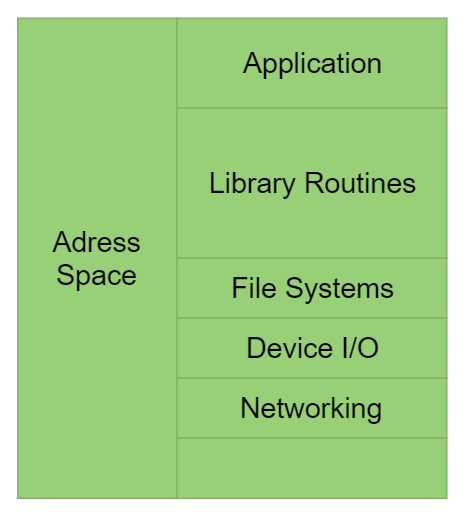
\includegraphics[width=0.2\textwidth]{unikernel_application_stack}
  \caption[Unikernel]{Unikernel application stack \cite{UnikernelSurvey}}
  \label{fig:unikernel_application_stack}
  \end{figure}

  \begin{figure}[htbp!] 
    \centering    
    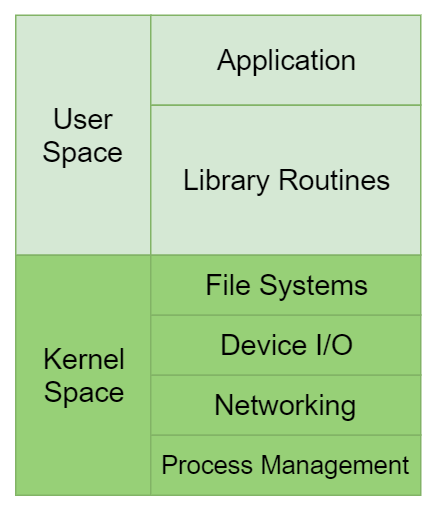
\includegraphics[width=0.2\textwidth]{normal_application_stack}
    \caption[Normal]{Normal application stack \cite{UnikernelSurvey}}
    \label{fig:normal_application_stack}
    \end{figure}

\subsubsection{Library Operating Systems}
Library\cite{LibraryOS} operating system is an method of constructing an operating system where the kernel modules  
required by an application is executed in the same address space as the application. The original goal 
of Library operating systems was to improve performance by enabling applications to manage resources according to 
their own needs, thereby allowing a high level of customizability. One of the major drawbacks for 
Library OS was support for various device drivers written for specific hardware. 

Nowadays, however, virtualization already provides an abstraction of the underlying hardware by exposing 
virtualized hardware drivers. This allows library OS implementations to support the generic virtual driver 
as opposed to attempting to support various hardware drivers.

% Definition of Unikernels 
% Primary Software Stacks the Unikernel is supported for 
% Diagram of Unikernels 


\subsection{Types of Unikernels}
% Library OS 
% Binary Compatible Uni-kernels 
\subsubsection{Clean slate (Specialized and purpose-built unikernels)}
Designed to utilize all the modern features of software and hardware, without worrying about backward
compatibility. They are not POSIX-compliant. 
\begin{itemize}
  \item Halvm (TODO survey)
  \item MirageOS (TODO survey)
\end{itemize}

\subsubsection{Legacy (Generalized "fat" unikernels)}
Designed to run unmodified applications in an Unikernel, 
which make them bulky in comparison to the clean slate approach. 
Designed to be POSIX compliant. The following below 
are the ones surveyed in the following paper: 
\begin{itemize}
  \item Unikraft
  \item OSv 
  \item HermitCore 
  \item RKOS
  \item Azelea
  \item IncludeOS 
  \item ClickOS
  \item NanoOS
\end{itemize}
%
% 4. Figures for all implementations 
% 5. References for all implementations 
% 6. Table analyses for all implementations 
% 7. More on Hermit core (Phrase research questions based on Hermit core)
%
\subsection{Implementations}

\subsubsection{Unikraft \cite{Unikraft}}
Unikraft is a uni-kernel implementation that claims to be 
a micro library OS. \emph{The major features of Unikraft is:}
\begin{itemize}
  \item Single address space: Intended to target single applications.
  \item Fully modular system: All drivers and platform libraries can be easily removed.
  \item Single protection level: No kernel and user space separation to avoid costly context switching.
  \item Static linking: Compiler features such as dead code elimination and link time optimization supported. 
  \item POSIX support: Support for legacy applications while still allowing for specialization. 
  \item Platform abstraction: The ability to run on different Hypervisors/VMs. 
\end{itemize}
\emph{To reach for the principal of modularity. Unikraft consists of 2 major components:}
\begin{itemize}
  \item Micro libraries: Micro-libraries are software components 
  which implement one of the core Unikraft APIs.
  \item Build system: The build system
  then compiles all of the micro-libraries, links them,
  and produces one binary per selected platform.
\end{itemize}
\emph{In terms of performance the following was evaluated in Unikraft:}
\begin{itemize}
  \item Resource Efficiency (Smaller is Better): Overall, the total VM boot time is dominated by the VMM,
  with Solo5 and Firecracker being the fastest (3ms), QEMU
  microVM at around 10ms and QEMU the slowest at around
  40ms.
  \item Filesystem Performance: Unikraft
  achieves lower read latency and lower write latency with
  different block sizes and are considerably better than ones
  from the Linux VM.
  \item Application Throughput: Unikraft is around 30\%-80\% faster than running the same app
  in a container, and 70\%-170\% faster than the same app running 
  in a Linux VM. Surprisingly, Unikraft is also 10\%-60\%
  faster than Native Linux in both cases.
  \item Performance of Automatically Ported Apps: The results
  show that the automatically ported app is only 1.5\% slower
  than the manually ported version, and even slightly faster
  than Linux bare-metal.
\end{itemize}

\begin{figure}[htbp!] 
  \centering    
  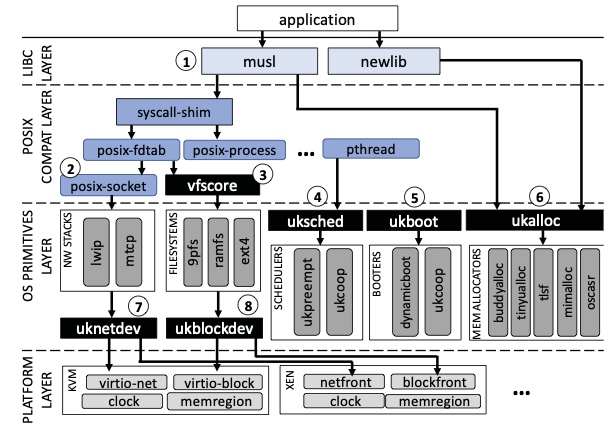
\includegraphics[width=0.6\textwidth]{UnikraftStack}
  \caption[Unikraft]{Unikraft application stack \cite{Unikraft}}
  \label{fig:UnikraftStack}
  \end{figure}
  % source https://dl.acm.org/doi/pdf/10.1145/3447786.3456248

\subsubsection{OSv}
OSv\cite{OSvPaper} is an Unikernel that runs existing Linux cloud applications on various hypervisors 
and machine architectures. OSv runs on 64-bit x86 and
ARM architectures and supports KVM/Qemu, VMware, Xen and VirtualBox 
hypervisors.OSv demonstrates up to 25\% increase in throughput and 47\% 
decrease in latency. 
By using non-POSIX network APIs,
it can further improve performance and demonstrate a
290\% increase in Memcached throughput.
OSv is designed as a drop-in replacement for applications that use a
supported subset of the Linux application binary interface (ABI).
\emph{The following below is the design of OSv:}
\begin{itemize}
  \item Memory Management: OSv uses virtual memory like
  general purpose OSs.OSv supports demand paging and memory mapping
  via the mmap API.
  \item No Spinlocks: The mutex implementation is based on a lock-free design 
  by Gidenstam \& Papatriantafilou \cite{LockFree}, which protects
  the mutex's internal data structures with atomic operations in a lock-free fashion.
  \item Network Channels: In OSv almost all packet processing is performed in an application thread. 
  Upon packet received, a simple classifier associates it with a channel, which is a single producer/single
  consumer queue for transferring packets to the application thread.
\end{itemize}

\begin{figure}[htbp!] 
  \centering    
  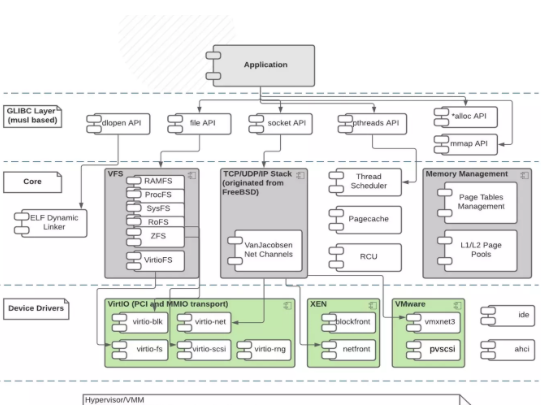
\includegraphics[width=0.7\textwidth]{OSvStack}
  \caption[OSv]{OSv application stack \cite{OSvDiagram}}
  \label{fig:OSv}
  \end{figure}
  % source https://www.slideshare.net/ScyllaDB/osv-unikernel-optimizing-guest-os-to-run-stateless-and-serverless-apps-in-the-cloud



\subsubsection{HermitCore}
HermitCore\cite{HermitCore} is an Unikernel implementation designed for HPC. The kernel extends the
multi-kernel approach with the advantages of a Unikernel.The focus of HermitCore is 
the mapping of the hardware to
the software structure rather than full support of the Linux
API.In a HermitCore system, each NUMA node runs its own HermitCore instance managing all its resources.
\emph{The aims for Hermit core are the following:}
\begin{itemize}
  \item Reduction of OS noise.
  \item Predictable runtimes.
  \item Maintainability, extensibility, and flexibility.
  \item Abstraction of hardware details.
  \item Support for common HPC programming models (e. g.,
  OpenMP, MPI).
  \item Simple integration into existing software stacks of
  compute centers.
\end{itemize}
\emph{Benchmarks conducted:}
\begin{itemize}
  \item Operating System Micro-Benchmarks.
  \item Hourglass Benchmark (For OS Noise).
  \item Inter-kernel Communication Benchmark.
  \item OpenMP Micro-Benchmarks.
\end{itemize}
\emph{The following are derived projects from the hermit-core project:}
\begin{itemize}
  \item HermitTux \cite{Hermitux} : It is a linux binary compatible Unikernel that can run native linux executables. 
  \item RustyHermit \cite{RustyHermit}: Implementation of the Hermit core Unikernel in Rust. 
  \item Lib-hermitMPK \cite{HermitMPK} : Providing support for IntelMPK for RustyHermit to isolate the unsafe parts of the kernel and 
  application with proven performance similar RustyHermit without the memory protection.
\end{itemize}
% \begin{itemize}
%   \item HermitTux : It is a linux binary compatible Unikernel that can run native linux executables. 
%   \item RustyHermit : Implementation of the Hermit core Unikernel in Rust. 
%   \item Lib-hermitMPK : Providing support for IntelMPK for RustyHermit to isolate the unsafe parts of the kernel and isolate 
%   the application with a similar performance of RustyHermit without the memory protection.
% \end{itemize}

\begin{figure}[htbp!] 
  \centering    
  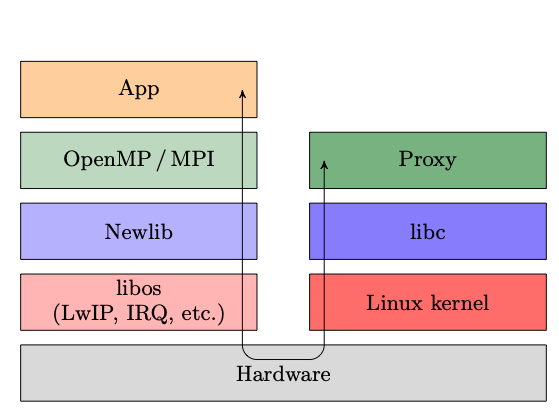
\includegraphics[width=0.5\textwidth]{HermitCoreStack}
  \caption[HermitCore]{HermitCore Software stack \cite{HermitCore}}
  \label{fig:HermitCoreStack}
  \end{figure}
  % source https://dl.acm.org/doi/pdf/10.1145/2931088.2931093

  \begin{figure}[htbp!] 
    \centering    
    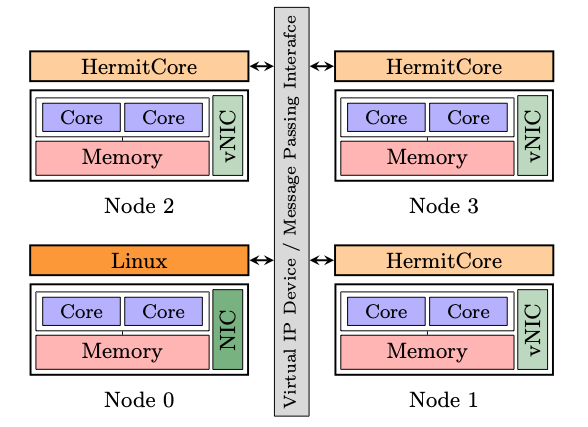
\includegraphics[width=0.8\textwidth]{NumaHermitCore}
    \caption[HermitCore]{A NUMA system with one satellite kernel per NUMA node \cite{HermitCore}}
    \label{fig:HermitCoreStack}
    \end{figure}
    % source https://dl.acm.org/doi/pdf/10.1145/2931088.2931093



\subsubsection{RKOS}
% source: https://media.taricorp.net/rkos.pdf
RKOS\cite{RKOS} is an unikernel implemented in Rust which
offers safety guarantees comparable to implementations which depend on complex runtime
libraries while being capable of providing predictable application performance demanded
by real-time applications in a relatively simple implementation. 
\emph{Design decisions for RKOS are as follows:}
\begin{itemize}
  \item Mutual trust between components allows a shared, uniform address space.
  \item Virtualized runtime environments have uniform hardware configuration.
\end{itemize}
\emph{Performance Evaluations conducted:}
\begin{itemize}
  \item Run time memory footprint 
  \item Binary size 
\end{itemize}

\subsubsection{ClickOS}
ClickOS\cite{ClickOS} is an unikernel optimized for middleboxes that runs exclusively on
the Xen hypervisor with small virtual machine memory footprint overhead
(5 MB), fast boot times (under 30 milliseconds), and high performance
networking capabilities.ClickOS adds only a 45 microsecond delay per
packet. When compared to a general purpose Linux also running on Xen,
ClickOS network throughput is up to 1.5x times higher for MTU-sized packets
and as much as 13.6x times higher for minimum-sized packets. 

\begin{figure}[htbp!] 
  \centering    
  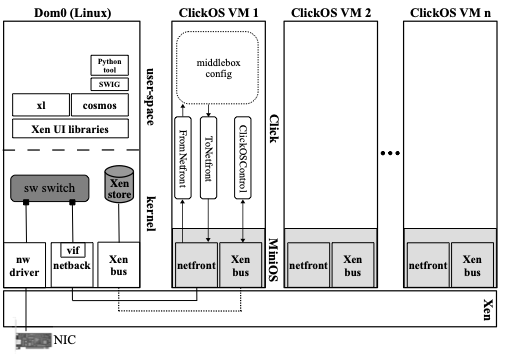
\includegraphics[width=0.6\textwidth]{ClickOSStack}
  \caption[ClickOS]{ClickOS architecture \cite{ClickOS}}
  \label{fig:ClickOSStack}
  \end{figure}
  % source https://www.usenix.org/system/files/conference/nsdi14/nsdi14-paper-martins.pdf

\subsubsection{NanoOS \cite{NanoOS}}
Nanos is a Unikernel implementation designed to run micro services on the 
Cloud, it runs on top of a Qemu Hypervisor and has it's own Orchestrator 
written in Go called OPS. 
Nanos employs various forms of security measures found in other general purpose operating systems including ASLR and respects page protections 
that the compilers produce.

\emph{ASLR:}

\begin{itemize}
  \item Stack Randomization
  \item Heap Randomization
  \item Library Randomization
  \item Binary Randomization
\end{itemize}

\emph{Page Protections:}

\begin{itemize}
  \item Stack Execution off by Default
  \item Heap Execution off by Default
  \item Null Page is Not Mapped
  \item Rodata no execute
  \item Text no write
\end{itemize}

\begin{itemize}
  \item SMEP
  \item UMIP
\end{itemize}

\emph{Performance Evaluations conducted:}
\begin{itemize}
  \item Bootup Times.
  \item Requests per second.
\end{itemize}

\subsubsection{IncludeOS}
IncludeOS\cite{IncludeOS} is a single tasking library operating system for 
cloud services which is written from scratch in C++. Key features include:
extremely small disk and memory footprint, efficient asynchronous I/O, 
OS-library where only what your service needs gets included.
In the test case the bootable disk image consisting
of a simple DNS server with OS included is shown
to require only 158 kb of disk space and to require
5-20\% less CPU-time.
\emph{The contributions of IncludeOS are:}
\begin{itemize}
  \item Extreme resource efficiency and footprint.
  \item Efficient deployment process.
  \item Virtualization platform independence.
\end{itemize}
\emph{The proposed benefits of IncludeOS  in comparison to Linux Kernels are:}
\begin{itemize}
  \item Extremely small disk and memory footprint.
  \item No host or software dependencies, other than
  virtual x86 hardware, and standard virtio for
  networking
  \item No system call overhead (The OS and the
  services are in the same binary, and the system calls
  are simple function calls(i.e without passing any
  memory protection barriers)).
  \item Reduced number of VMs exits by keeping the
  number of protected instructions very low.
\end{itemize}

\emph{Performance Evaluations conducted:}
\begin{itemize}
  \item Bootup times 
  \item Memory performance (i.e The Stream Benchmark)
\end{itemize}

\subsubsection{Azelea}
Azalea\cite{Azelea} is a multi-kernel OS, which consists of Unikernels and a full kernel. Azelea Unikernel provides scalability and parallel performance. 
The full kernel provides compatibility with POSIX APIs that the Unikernel cannot handle. The Full kernel is combined with the Unikernel for 
side by side partitioning. \emph{The Azelea Unikernel is a library OS which consists of the following:}
\begin{itemize}
  \item Kernel Functions 
  \item Run time libraries 
  \item Application 
\end{itemize}
A server can run multiple Azelea-unikernels with the number of cores and memory allocated. The Linux install which is a part of 
the server acts as a driver and that loads each Unikernel or supports communication between other nodes. 
\emph{The contributions of Azelea Uni-kernels are:}
\begin{itemize}
  \item Lightweight kernel.
  \item Compatibility with legacy application (i.e Support for statically build Linux binaries).
  \item I/O offloading (i.e FWK(Full weight kernel) handles all the I/O offloading so that applications can be executed without any interference). 
\end{itemize}

\emph{Performance Evaluations conducted:}
\begin{itemize}
  \item OS Noise (FTQ, FWQ, Hour Glass) \cite{AzeleaOSNoise}
  \item IO offload acceleration \cite{AzeleaIOAccerleration}
\end{itemize}

\begin{figure}[htbp!] 
  \centering    
  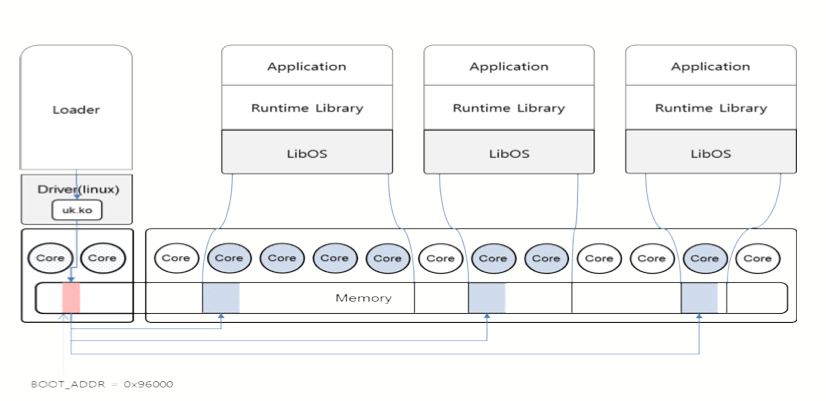
\includegraphics[width=0.6\textwidth]{AzeleaKNL}
  \caption[Azelea]{Azelea-unikernel in a single KNL \cite{Azelea}}
  \label{fig:AzeleaKNL}
  \end{figure}
  % source https://ieeexplore.ieee.org/stamp/stamp.jsp?tp=&arnumber=8539634

\subsubsection{HaLVM}
HaLVM(Haskell Lightweight Virtual machine) is an unikernel implementation based on Xen hypervisor (i.e type 1 hypervisor). 
HaLVM is implemented using Haskell. HaLVM is suitable for small, single-use and
low-dependence programs. There was only 1 published work was a paper on analyzing 
parallel programs model for HaLVM\cite{HaLVM}. 

% \emph{Performance Evaluations conducted(parallel model):}
% \begin{itemize}
%   \item Eval monad
%   \item forkIO
%   \item forkOS
%   \item Cloud Haskell
%   \item IVC
% \end{itemize}

\begin{figure}[htbp!] 
  \centering    
  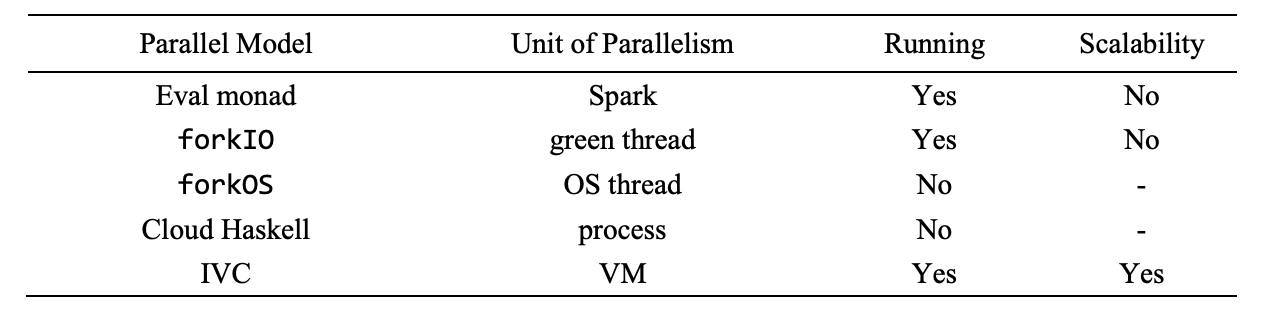
\includegraphics[width=0.8\textwidth]{halvm-execution}
  \caption[halvm-execution]{Performance Evaluations conducted(parallel model) \cite{HaLVM}}
  \label{fig:HaLVM}
  \end{figure}

\begin{figure}[htbp!] 
  \centering    
  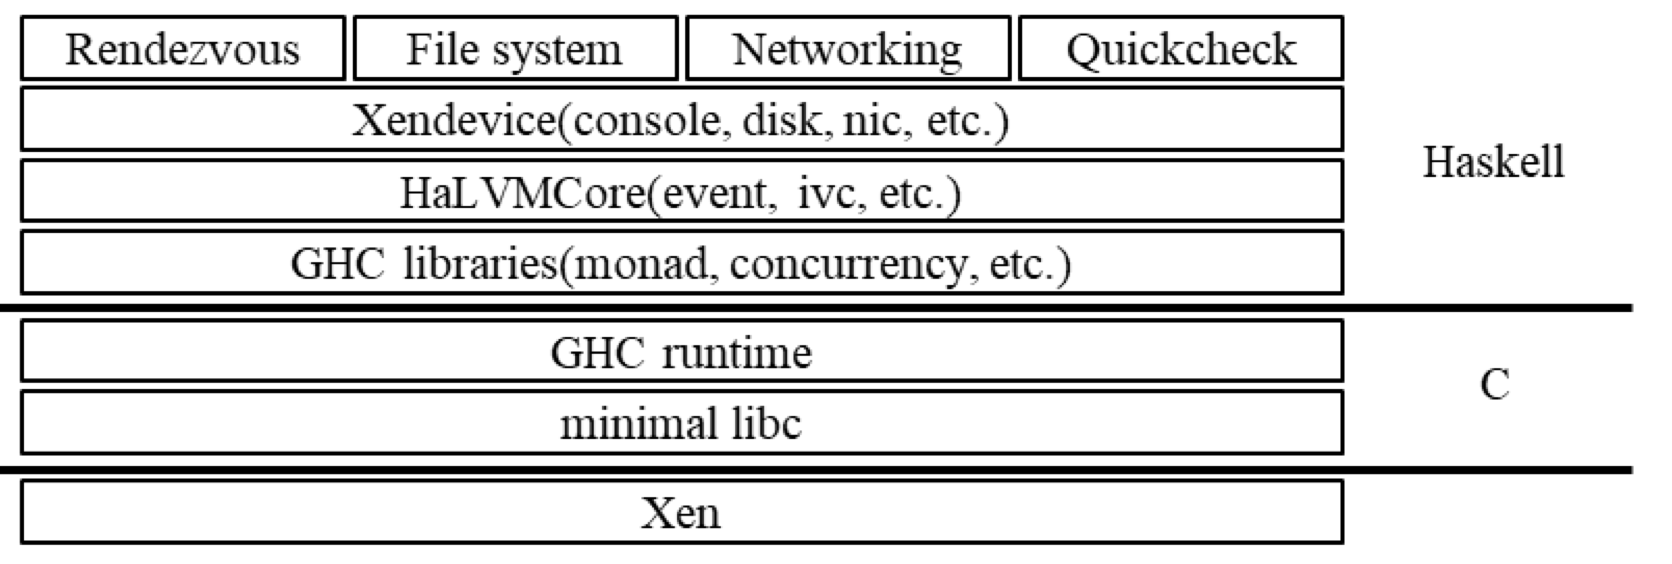
\includegraphics[width=0.6\textwidth]{halvm}
  \caption[HaLVM]{HaLVM architecture \cite{HaLVM}}
  \label{fig:HaLVM}
  \end{figure}

  \subsubsection{Mirage}
  Mirage\cite{mirage} produces an Unikernel by compiling and 
  linking OCaml to an Xen VM image. The objective 
  was to combine static type-safety with a single
  address-space layout. Using Mirage it is possible 
  to use libraries such as networking, storage and concurrency
  that works under unix during development, when compiled 
  to production becomes operating system drivers. 

  \emph{Mirage takes advantage of Ocaml for the following reasons:}
  \begin{itemize}
    \item Static type checking
    \item Automatic memory management
    \item Modules
    \item Metaprogramming
  \end{itemize}

  \emph{Performance Evaluations conducted:}
  \begin{itemize}
    \item Boot time.
    \item Thread performance.
    \item Throughput.
    \item Sessions per for a sample dynamic web application.
  \end{itemize}
  
  \begin{figure}[htbp!] 
    \centering    
    \includegraphics[width=0.6\textwidth]{Mirage}
    \caption[Mirage]{Azelea-unikernel in a single KNL \cite{Azelea}}
    \label{fig:Mirage}
    \end{figure}

\subsection{Unikernel analysis}
The following section consists of analysis of the Uni-kernels 
implementations surveyed in the current literature. The 
analyses is based on: 
\begin{itemize}
\item Best suitable implementations for various platforms supported ? 
% \item Best suitable for various architectures ?
% \item Best implementation in terms of performance ?
\item How do each of them handle parallel applications ?
% \item Best tools with the most concrete evaluation ? 
\end{itemize}


% \begin{table}[]
%   \resizebox{\columnwidth}{!}{%
%   \begin{tabular}{@{}|l|l|l|l|@{}}
%   \toprule
%   \textit{\textbf{Unikernel}} & \textit{\textbf{Languages supported}}                                                                   & \textit{\textbf{Targets}}                                                                            & \textbf{Performance evaluation}                                                                                                                                                                                                                   \\ \midrule
%   \textit{Unikraft\cite{Unikraft}}           & \textit{C, C++, Rust, Go, Python}                                                                       & \textit{\begin{tabular}[c]{@{}l@{}}KVM, Xen, Linux Userspace, Solo5, \\ VMware, HyperV\end{tabular}} & \begin{tabular}[c]{@{}l@{}}- Resource \\   Efficiency \\ - Filesystem \\   Performance \\ - Application \\   throughput. \\ - Performance of \\   Automatically ported \\   apps.\end{tabular}                                                    \\ \midrule
%   OSv\cite{OSvPaper}                         & Java, C, C++, Node, Ruby, Go                                                                            & Virtual Box, EXSi, KVM and HyperV.                                                                   &                                                                                                                                                                                                                                                   \\ \midrule
%   NanoOS\cite{NanoOS}                     & \begin{tabular}[c]{@{}l@{}}C, C++, Go, Java, Node js, Python, \\ Rust, Rust, Ruby, and PHP\end{tabular} & \begin{tabular}[c]{@{}l@{}}KVM, XEN,ESXi and \\ Hyper V\end{tabular}                                 & \begin{tabular}[c]{@{}l@{}}- Boot Up \\    times \\ - Request \\   per second\end{tabular}                                                                                                                                                        \\ \midrule
%   HermitCore\cite{HermitCore}                  & Rust, C,C++, Go and Fortran                                                                             & uhyve, KVM and bare metal                                                                            & \begin{tabular}[c]{@{}l@{}}- Operating system \\   micro benchmark\\ - Hourglass benchmark \\ - Inter-kernel \\   communication benchmark \\ - OpenMP micro benchmark\end{tabular}                                                                \\ \midrule
%   RKOS\cite{RKOS}                        & Rust                                                                                                    & Bare metal                                                                                           & \begin{tabular}[c]{@{}l@{}}- Run time \\   memory footprint \\ - Binary size\end{tabular}                                                                                                                                                         \\ \midrule
%   ClickOS\cite{ClickOS}                     & C++                                                                                                     & Xen                                                                                                  & \begin{tabular}[c]{@{}l@{}}- ClickOS Switch \\ - Memory Footprint \\ - Boot times \\ - Delay (When processing packets)\\ - Throughput (Amount of packets \\    ClickOS can handle)\\ - State Insertion \\ - Chaning \\ - Scaling out\end{tabular} \\ \midrule
%   IncludeOS\cite{IncludeOS}                   & C++                                                                                                     & KVM, VirtualBox, ESXi, OpenStack                                                                     & \begin{tabular}[c]{@{}l@{}}- Bootup times \\ - Memory Performance\end{tabular}                                                                                                                                                                    \\ \bottomrule
%   \end{tabular}%
%   }
%   \end{table}

% Please add the following required packages to your document preamble:
% \usepackage{graphicx}
% \usepackage{lscape}
\begin{landscape}
  \begin{table}[]
  \caption{Analyzing various Uni-kernel implementations}
  \label{tab:unikerneltable}
  \resizebox{\columnwidth}{!}{%
  \begin{tabular}{llll}
  \hline
  \multicolumn{1}{l|}{\textbf{Unikernel}} & \multicolumn{1}{l|}{\textbf{Languages supported}} & \multicolumn{1}{l|}{\textbf{Targets}} & \textbf{Performance evaluation} \\ \hline
  \multicolumn{1}{l|}{Unikraft} & \multicolumn{1}{l|}{C, C++, Rust, Go, Python} & \multicolumn{1}{l|}{KVM, Xen, Linux Userspace, Solo5, VMware, HyperV} & \begin{tabular}[c]{@{}l@{}}- Resource  Efficiency \\ - Filesystem Performance\\ - Application throughput. \\ - Performance of  Automatically ported apps.\end{tabular} \\ \hline
  \multicolumn{1}{l|}{OSv} & \multicolumn{1}{l|}{Java, C, C++, Node, Ruby, Go} & \multicolumn{1}{l|}{Virtual Box, EXSi, KVM and HyperV.} & \begin{tabular}[c]{@{}l@{}}-  Macro Benchmarks (Memcached, SPECjvm2008)\\ -  Micro Benchmarks (Network performance, \\    JVM ballon, \\    context switches)\end{tabular} \\ \hline
  \multicolumn{1}{l|}{NanoOS} & \multicolumn{1}{l|}{C, C++, Go, Java, Node js, Python,  Rust, Ruby, and PHP} & \multicolumn{1}{l|}{KVM, XEN,ESXi and Hyper V} & \begin{tabular}[c]{@{}l@{}}- Boot Up times \\ - Request per second\end{tabular} \\ \hline
  \multicolumn{1}{l|}{HermitCore} & \multicolumn{1}{l|}{Rust, C, C++, Go and Fortran} & \multicolumn{1}{l|}{uhyve, KVM and bare metal} & \begin{tabular}[c]{@{}l@{}}- Operating system micro benchmark\\ - Hourglass benchmark \\ - Inter-kernel communication benchmark \\ - OpenMP micro benchmark\end{tabular} \\ \hline
  \multicolumn{1}{l|}{RKOS} & \multicolumn{1}{l|}{Rust} & \multicolumn{1}{l|}{Bare metal} & \begin{tabular}[c]{@{}l@{}}- Run time memory footprint \\ - Binary size\end{tabular} \\ \hline
  \multicolumn{1}{l|}{ClickOS} & \multicolumn{1}{l|}{C++} & \multicolumn{1}{l|}{Xen} & \begin{tabular}[c]{@{}l@{}}- ClickOS Switch \\ - Memory Footprint \\ - Boot times \\ - Delay (When processing packets)\\ - Throughput (Amount of packets ClickOS \\    can handle)\\ - State Insertion\\ - Chaining \\ - Scaling out\end{tabular} \\ \hline
  \multicolumn{1}{l|}{IncludeOS} & \multicolumn{1}{l|}{C++} & \multicolumn{1}{l|}{KVM, VirtualBox, ESXi, OpenStack} & \begin{tabular}[c]{@{}l@{}}- Bootup times \\ - Memory Performance\end{tabular} \\ \hline
  Azelea & C & Bare-metal & \begin{tabular}[c]{@{}l@{}}- OS Noise (FTQ, FWQ, Hour Glass)\\ - IO offload acceleration\end{tabular}
  \end{tabular}%
  }
  \end{table}
  \end{landscape}

\subsubsection{Best suitable implementations based on platforms(i.e targets) supported ?}
This refers to which Uni-kernel implementation would be preferred based on the various targets supported, this is 
based on table \ref{tab:unikerneltable}. Based on the number of targets supported Unikraft has the most amount of 
targets supported. Since the the research goals (//todo refer research goals) for using Uni-kernels is to run on 
bare-metal as a major requirement (This is because of the way multi-kernels work~\ref{Multi-kernels} ).Unikraft would be suitable for testing a multi-kernel environment, but porting to 
bare-metal would be an important step along the way. Hermit-core would be suitable since it does support running 
on bare-metal and runs on a hypervisor (i.e KVM and uhyve). 

% \subsubsection{Best suitable for various architectures ?}
\subsubsection{Multi-core}
\underline{Unikraft} does not currently support Multi-core mode yet. By default it uses the library
uklock which synchronization primitives such as Mutexes and semaphores. If multi-core 
was supported primitives such as spin-locks and RCUs would be supported. 
\hfill \break

\underline{OSv} supports running application in multiple cores. OSv thread scheduler is lock-free, 
preemptive, tick-less, fair, scalable and efficient. 
\begin{itemize}
  \item Lock-free: The scheduler keeps separate run-queue on CPU. Sleeping threads 
  are not listed on any run-queue. Separate run queues leads to a situation where 
  one CPUs queue has more runnable threads than another CPUs queue, this impacts 
  the scheduler. This is solved by a load balancer thread on each CPU. 
  \item Preemptive: OSv supports preemptive multi-tasking. According to the 
  paper\cite{OSv} this feature is useful for maintaining per-CPU variables and 
  RCU locks. 
  \item Tick-less: OSv uses a high resolution clock, scheduler accounts to each thread 
  the exact time it consumed, this is in-contrast to approximating ticks. 
  \item Fair: On each reschedule, the scheduler must decide which of the CPUs runnable 
  threads should run next and for how long. OSv scheduler calculates the exponentially-decaying 
  moving average of each thread's recent run time. The scheduler decides the next runnable 
  thread with the lowest moving-average runtime.
  \item Scalable: OSv scheduler has O(log N) complexity in the number of runnable threads on 
  each CPU.
  \item Efficient: Apart from the scheduler scalability, OSv employs additional techniques to 
  make the scheduler and context switches more efficient. OSv single address space 
  means there is no need to switch page tables and or flush the TLB on context switches. 
  This means that context switches are significantly cheaper than the standard 
  multi-process operating system.
\end{itemize}
\hfill \break

\underline{HermitCore} (i.e currently called RustyHermit) supports multi-threaded and 
multiprocessing applications. The scheduler does not support load balancing 
this is because explicit thread placing is preferred over automatic 
strategies. The scheduling overhead is also minimized by employing a 
dynamic timer (i.e the kernel does not interrupt computational threads which runs on 
particular cores and due to this a timer is not needed).
\hfill \break

\underline{RKOS} supports concurrency and multi-threading. The threads are preemptive and scheduled non-cooperatively.
Preemptive multitasking was selected because it was largely used with existing systems. 
\hfill \break

\underline{Azelea} Unikernel supports multi threaded applications. Each core uses a queue to manage multiple threads 
and with a round robin scheduler. 

% \subsubsection{Best tools with the most concrete evaluation ? }

% Compare Unikraft and HermitCore (i.e Rusty hermit)


% ------------------------------ Multi-kernel --------------------------------

\section[Multi-kernels]{Multi-kernels Survey}
\label{Multi-kernels}
The following is the survey for Multi-kernels. The introduction is 
based on the first paper published on Multi-kernels \cite{multi_kernel_first_paper},
follows up with a survey on various implementations and with an 
analysis section of various multi-kernel implementation. 


\subsection{Introduction to Multi-kernels}
"A multikernel operating system treats a multi-core machine as a network of independent cores, as if it were a distributed system" \cite{Multi_kernel_wikipedia}.
It implements interprocess communications as message-passing. The design of multi-kernels can be stated as the following: 
\begin{itemize}
  \item Inter-core communication is explicit. 
  \item OS Structure is hardware neutral.
  \item State is view as replicated instead of shared.
\end{itemize}

\begin{figure}[htbp!] 
  \centering    
  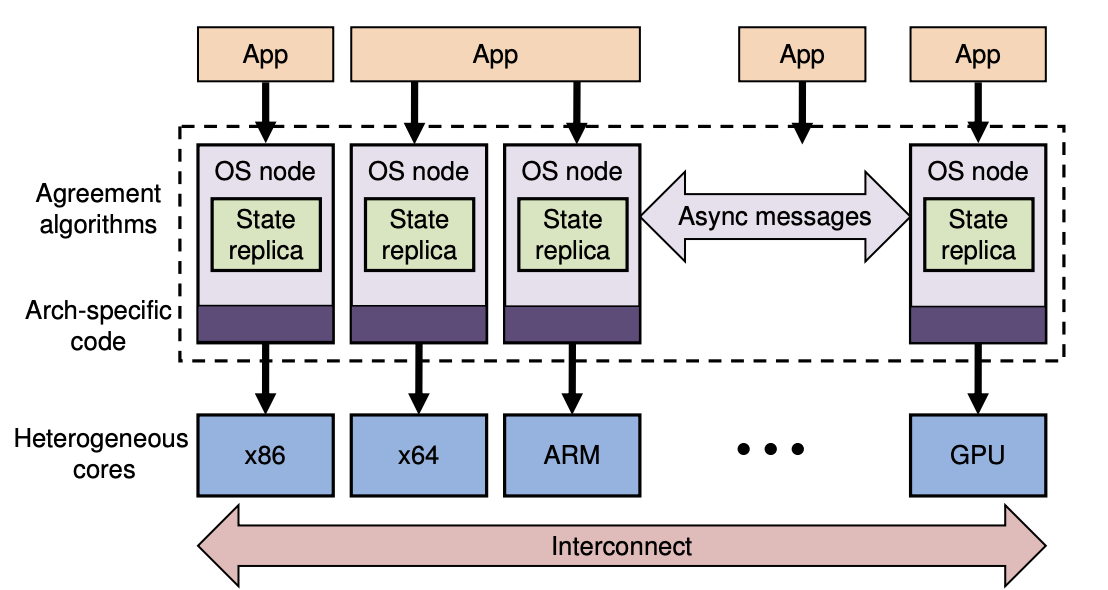
\includegraphics[width=0.6\textwidth]{Multi-kernel}
  \caption[Multi-kernel]{The Multi-kernel model \cite{multi_kernel_first_paper}}
  \label{fig:AzeleaKNL}
  \end{figure}

\subsubsection{Benefits of Multi-kernels}
The following below highlights the major characteristics
of Multi-kernels. 

\begin{itemize}
  \item Ability to handle diverse set of cores: 
  \item Interconnect matters: 
  \item Messages cost less than shared memory:
\end{itemize}

\subsection{Implementation}
The following section mentions about the Multi-kernel
implementations. 

\subsubsection{Barrelfish}
Barrelfish\cite{multi_kernel_first_paper} is a multi-kernel operating system that consists of a small kernel 
running on each core. The kernels share no memory (even on 
machines with cache-coherent shared RAM). A CPU 
driver in Barrelfish represents a kernel when is ran 
on a given core. In a heterogeneous system the CPU 
driver would different based on the architecture
of the core. 
% Add image 

\subsection{Popcorn Linux}
% https://www.kernel.org/doc/ols/2014/ols2014-barbalace.pdf
Popcorn\cite{PopcornLinux} linux is a replicated-kernel OS based on Linux. Popcorn 
boots up multiple instances of Linux kernels on a 
multi-core hardware. Popcorn linux was evaluated 
based on the NAS benchmark \cite{NAS}. 
% todo add more context about approach 
% todo Add image 

\subsection{FusedOS}
% Todo what is ran on the light weight cores 
FusedOS was one of the first to combine 
linux with a LWK(Light weight kernel). FusedOS 
was assuming heterogeneous hardware architecture 
that consists of both a light weight and full 
weight cores. The full cores runs linux and 
is also responsible to partition hardware 
resources between itself and LWKs.
To execute an application the LWK requests 
hardware resources (i.e light weight cores and memory) 
from the FWK(Full weight Kernel, This refers to the 
linux kernel). The system calls are generated 
by the application and are forwarded to Linux 
which is then handled with LWK process. 
% todo look at Github implementation 

\subsection{IHK/McKernel}
IHK/McKernel is a multi-kernel approach 
which runs Linux and LWKs side by side on 
compute nodes. A low-level software infrastructure
which is present at the heart of the stack 
which is called Interface for Heterogeneous
Kernels (IHK). By using IHK it is 
possible to dynamically partition resources 
in a many-core environment. An IKC (Inter-Kernel 
communication) layer is also introduced upon which 
the system call delegation is implemented. 
McKernel is a light weight kernel written 
from scratch and designed for HPC. McKernel
retains a binary compatible ABI with Linux. 
It supports multi-threading with a simple 
round robin cooperative scheduler. 

% \subsection{mOS}
% mOS creates a m

\subsection{FFMK}
FFMK (Fast and fault tolerant Microkernel based system) which 
is designed for Exascale computing. It investigates 
the feasibility of a Microkernel based hybrid OS designed 
for HPC.It relies on a L4 microkernel and a para-virtualized
Linux instance (i.e L4Linux\cite{l4linux}).
The idea of FFMK is to run HPC application directly on 
L4 with transparent access to linux features by using 
L4Linux. The L4Linux user process can be decoupled 
from the linux kernel and moved to another core 
if required (i.e by using the L4 Thread).

% \subsection{Hobbes}
% todo read: https://link.springer.com/chapter/10.1007/978-981-13-6624-6_15


% \subsection{Pisces/Kitten}

% \subsection{Kitten/Palacios}




% Major features 
% Implementation 
% upto 4 major ones 



% ------------------------------ Best suited for various architectures -----------------------------

\section[TAG based architecture survey]{TAG based architecture survey}   
The following was a survey conducted on existing TAG based implementations and the 
recent survey based on TAG based architectures \cite{acmTAGSurvey} published
in 2022 was a good staring point to understand about various implementations of TAG
based architectures with the high level merits and limitations. The following section 
provides our own version of the Survey to help decide the best implementations 
to answer the research questions (//TODO reference research questions chapter).

\subsection{Introduction to TAG based architectures}

Before deep diving into TAG based architecture implementations it is important to 
answer what is a TAG based architecture ? and the high level of various 
categories of various TAG based architectures.

Tagged architectures are a prominent class of hardware security primitives that augment data and code words
with tags. The tags, which function as the security metadata
about memory, are created before the program is loaded. 
Then, at runtime, the hardware enforces security policies on the tags to provide safety guarantees. 
The advantage being tags automate the secure and efficient management of security metadata. 

Tags policies as designed to address mostly:
\begin{itemize}
  \item Type and memory corruption
  \item Integer overflows
  \item Thread safety
  \item Buffer overflows
\end{itemize}

TAG policies can be categorized into 5 main categories which is:
\begin{itemize}
  \item Information-low control (IFC) policies
  \item Dynamic information-low tracking (DIFT) policies
  \item Capability models
  \item Programmable architectures
\end{itemize}

\subsection{Implementations}
 
According to the TAG based architecture survey \cite{acmTAGSurvey} there are 37 published
efforts on TAG based architectures over the past decade and 20 published efforts preceding that. 
The following below are relevant papers in relation to the research questions: 

\subsubsection{Timder V}
 Timber V\cite{weiser_timber-v_2019} is a tagged memory architecture for flexible and efficient isolation of code and data on 
 small embedded systems. The TAG isolation is augmented with a memory protection unit to isolate 
 individual processes. Timber V is compatible with existing code. The contributions of the paper 
 are: 
 \begin{itemize}
  \item Efficient tagged memory architecture for isolated execution on low-end processors. 
  \item Concept introduced called stack interleaving that allows efficient and dynamic memory management. 
  \item Lightweight shared memory between enclaves. 
  \item Efficient shared MPU (i.e Memory Protection Unit) design. 
 \end{itemize}

 \begin{figure}[htbp!] 
  \centering
  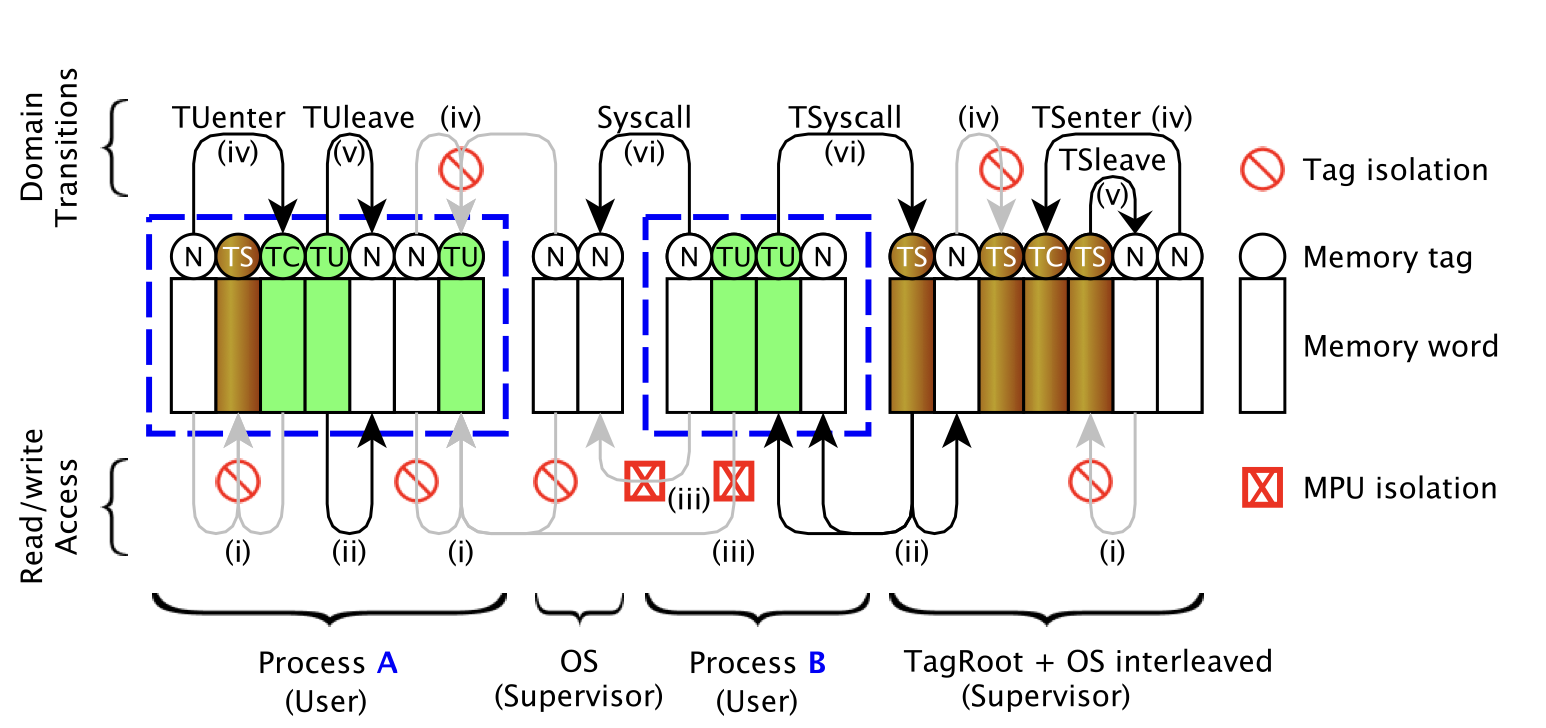
\includegraphics[width=0.6\textwidth]{Timber-V}
  \caption[MTE]{TimberV TAG interleaved on flat physical memory\cite{weiser_timber-v_2019}}
  \label{fig:MTE}
  \end{figure}
	
\subsubsection{ARM MTE}
The ARMv8.5-Memory Tagging Extension (MTE)\cite{ARMMTE} aims to increase the memory safety written for 
unsafe languages without requiring source code changes and in certain cases without 
recompilation. It generally focuses on the bounds checking use case, Though it 
provides limited tags which means it can only provide probabilistic overflow detection. 
It is one of the latest commercial incarnations of memory-safety-focused tagged architectures.   

\begin{figure}[htbp!] 
  \centering    
  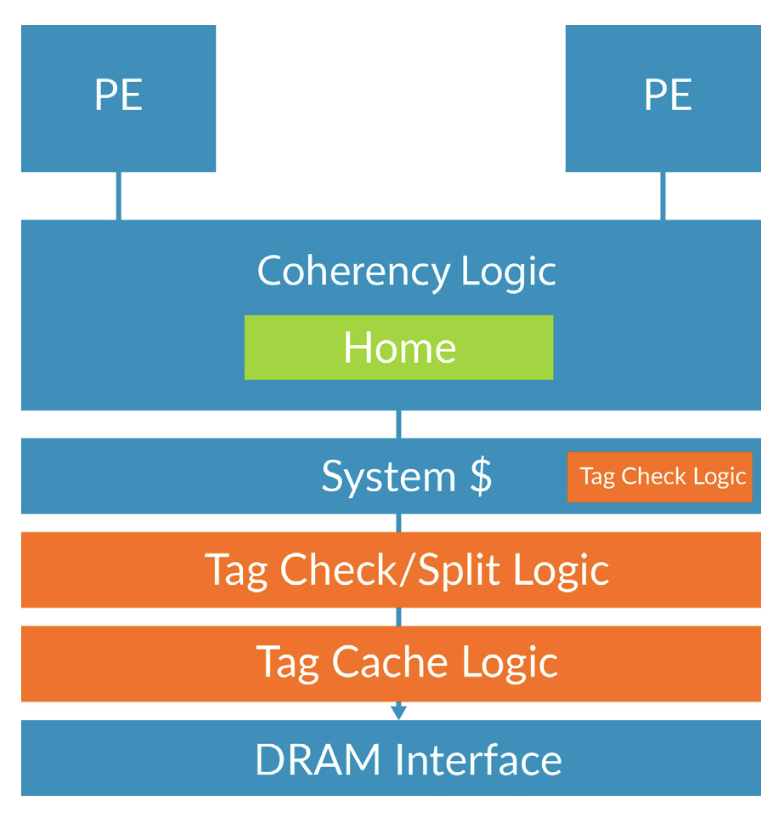
\includegraphics[width=0.2\textwidth]{ARMMTE}
  \caption[MTE]{Example of an ARM MTE-based system \cite{ARMMTE}}
  \label{fig:MTE}
  \end{figure}

\subsubsection{D-RI5CY}
D-RISCY\cite{D-RISCY} provides a design a design and implementation of a hardware dynamic information flow 
tracking (DIFT) architecture for RISC-V processor cores. The paper presents a low 
overhead implementation of DIFT that is specialized for low-end embedded systems
for IOT applications. The following are high level contributions:
\begin{itemize}
  \item Design f D-RI5CY, A DIFT-protected implementation of the RI5CY processor core. 
        The paper implements the modification of the DIFT TAG propagation and TAG checking
        mechanism in a way that is transparent to the execution of the regular instructions. 
  \item Concept introduced called stack interleaving that allows efficient and dynamic memory management.
  \item Lightweight shared memory between enclaves.
  \item Efficient shared MPU (i.e Memory Protection Unit) design.
\end{itemize}

\begin{figure}[htbp!] 
  \centering    
  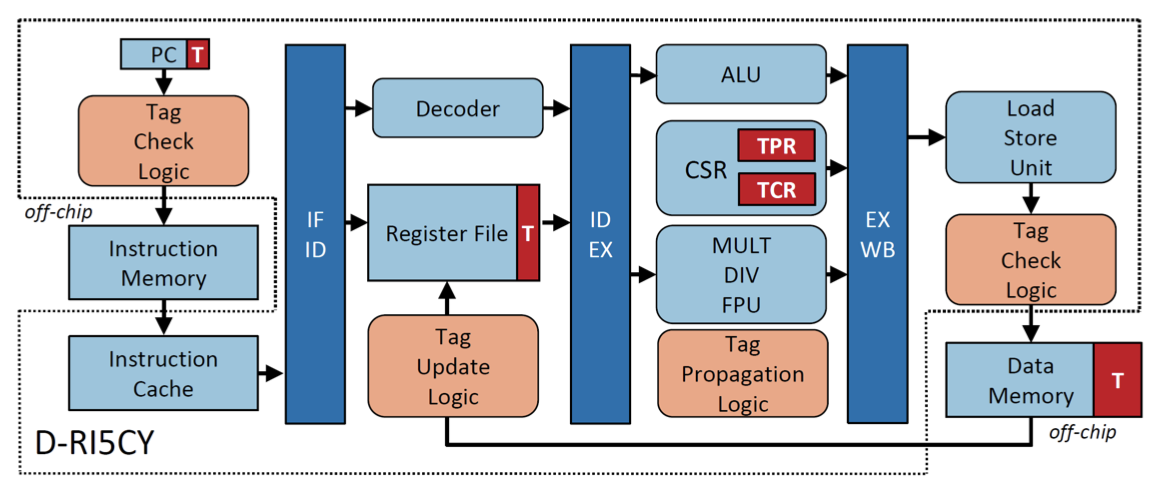
\includegraphics[width=0.6\textwidth]{D-RISCV}
  \caption[D-RISCY]{ Block diagram of the D-RI5CY processor. In red and pink the DIFT components. \cite{D-RISCY}}
  \label{fig:MTE}
  \end{figure}

%\subsection{TMDFI}


\subsubsection{HyperFlow} 
Hyperflow\cite{HyperFlow} is a design and security implementation that offers security assurance because it is implemented 
using a security-typed hardware description language. It allows complex information flow policies to 
be configured at run time. The paper introduces ChiselFlow, a new secure hardware description language. 
The contribution of the paper includes: 
\begin{itemize}
  \item Processor architecture and implementation designed for timing-safe information flow security. 
  \item Complete RISC-V instruction set extended with instructions for information flow control. 
  \item Verified at design time with a hardware description language. 
  \item Novel representations of lattices that can be implemented in hardware efficiently. 
\end{itemize}
HyperFlow implements a nonmalleable IFC policy using tags.
To eliminate timing side channels, the processor tracks the tag of the currently executing code and lushes caches,
TLB, branch predictor, and other micro-architectural state on changes in the conditionality or integrity tag of the
running code. The modifications to avoid timing side channels seem more extensive than those to add tags. The
authors report overheads in cycles per instruction of between 1\% and 69\%, largely due to padding the multiply
operation to the worst-case number of cycles.

\subsubsection{SDMP}
SDMP\cite{Sdmp} paper focuses on designing metadata tag based stack-protection security policies for general purpose tagged
architecture. The policies specifically
exploit the natural locality of dynamic program call graphs to
achieve cache-ability of the metadata rules that they require.
The simple Return Address Protection policy has a performance
overhead of 1.2\% but just protects return addresses.
The two richer policies present, Static Authorities and Depth Isolation, 
provide object-level protection for all stack objects. When
enforcing memory safety, The Static Authorities policy has a
performance overhead of 5.7\% and the Depth Isolation policy
has a performance overhead of 4.5\%.
The contribution of the paper includes:
\begin{itemize}
  \item The formulation of a range of stack protection policies
within the SDMP model.
  \item Three optimizations for the stack policies: Lazy Tagging,
Lazy Clearing and Cache Line Tagging.
  \item The performance modeling results of the policies on
a standard benchmark set, including the impact of the
proposed optimizations.
\end{itemize}

\subsubsection{Typed Architecture}
This paper introduces Typed
Architectures\cite{TypedArchitecture}, a high-efficiency, low-cost execution substrate 
for dynamic scripting languages, where each data
variable retains high-level type information at an ISA level.
Typed Architectures calculate and check the dynamic type
of each variable implicitly in hardware, rather than explicitly
in software. Typed Architectures provide
hardware support for flexible yet efficient type tag extraction
and insertion, capturing common data layout patterns of tag-
value pairs. The evaluation using a fully synthesizable RISC-
V RTL design on FPGA shows that Typed Architectures
achieve mean speedups of 11.2\% and 9.9\% with
minimum speedups of 32.6\% and 43.5\% for two production-
grade scripting engines for JavaScript and Lua. 
The contribution of the paper includes:
\begin{itemize}
  \item ISA extension to efficiently manage
type tags in hardware, which can be flexibly applied to
multiple scripting languages and engines.
  \item Design and implement the Typed Architecture pipeline,
which effectively reduces the overhead of dynamic type
checking at low hardware cost.
  \item Prototype the proposed processor architecture using 
a fully synthesizable RTL model to execute two
production-grade scripting engines with large inputs on
FPGA (executing over 274 billion instructions in total)
and provide a more accurate estimate of area and power
using a TSMC 40nm standard cell library.
\end{itemize}

\begin{figure}[htbp!] 
  \centering    
  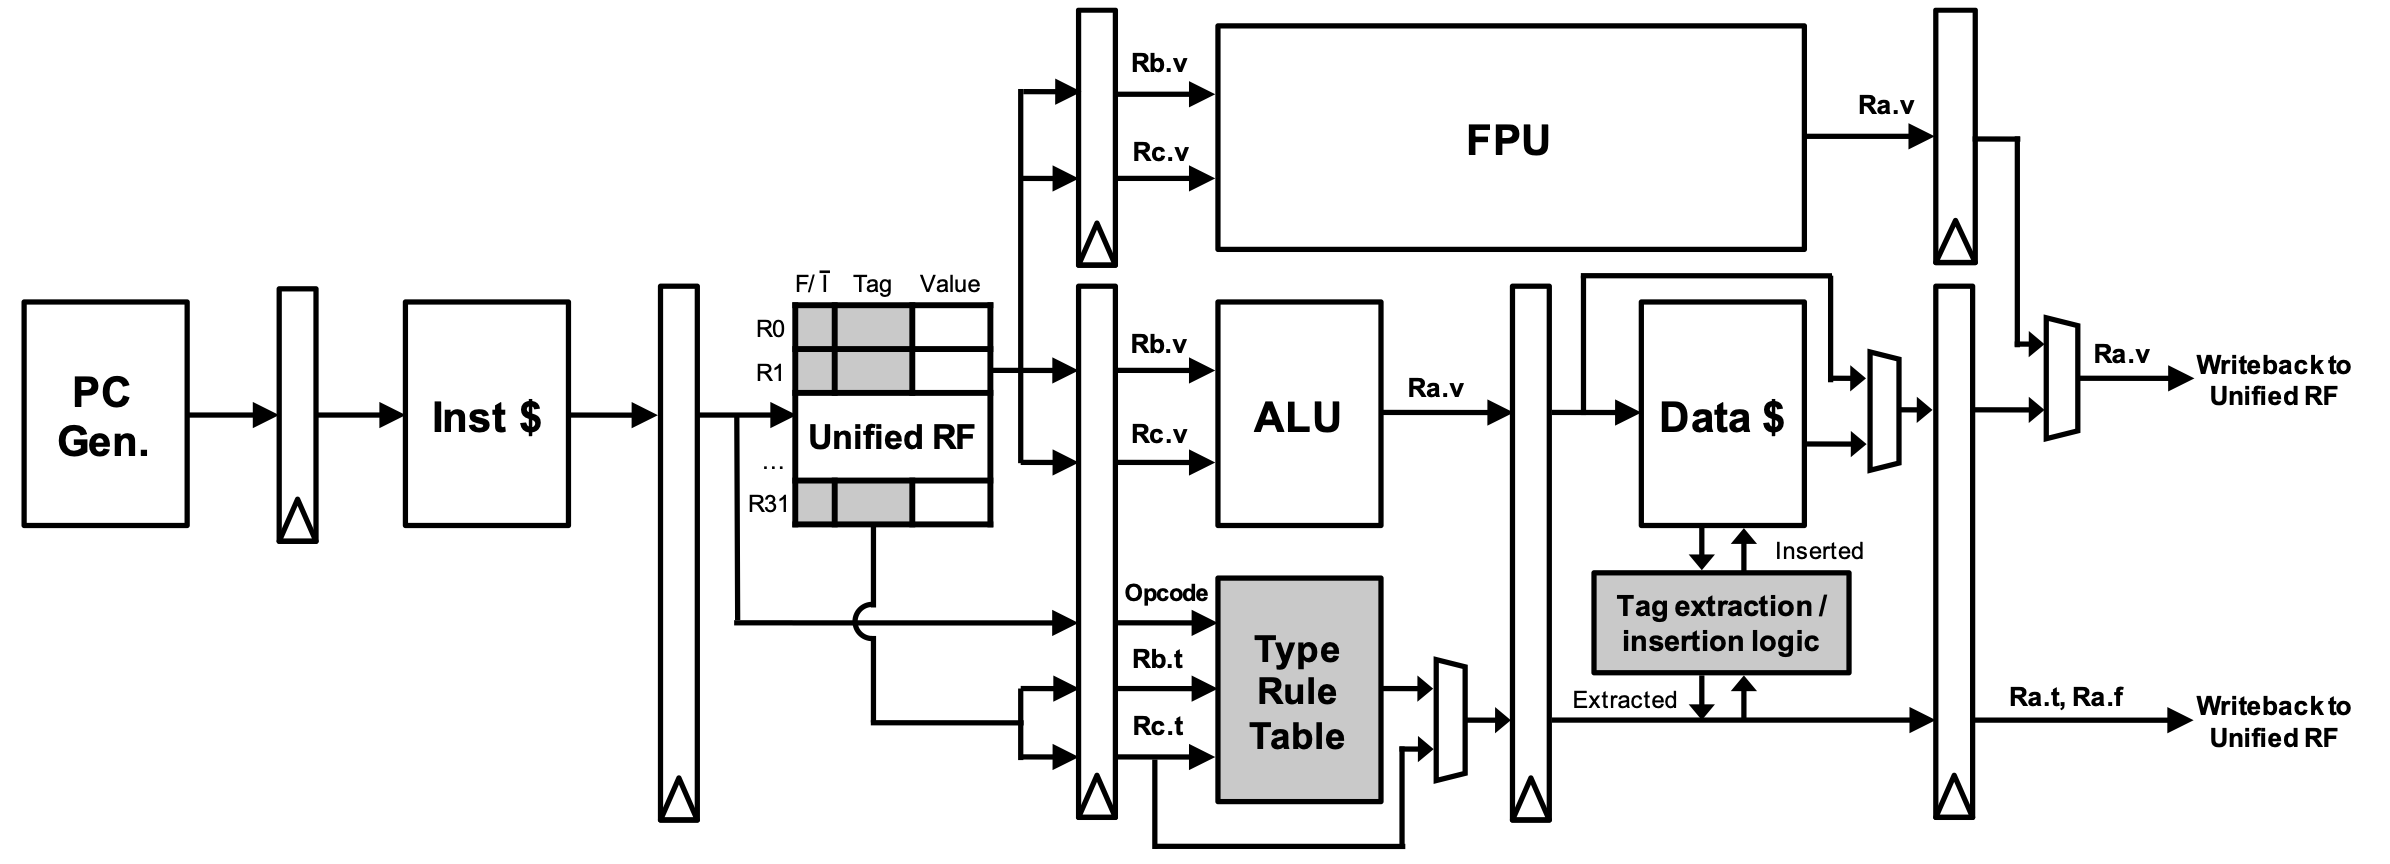
\includegraphics[width=0.8\textwidth]{TypedArchitecture}
  \caption[TypedArchitecture]{Pipeline structure augmented with Typed Architecture \cite{TypedArchitecture}}
  \label{fig:TypedArchitecture}
  \end{figure}

\subsubsection{Dover}
Dover\cite{Dover} is a secure processor that extends the conventional CPU with
a Policy Execution co-processor (PEX). PEX maintains metadata 
of every word assessable by the application processor. PEX 
enforces software-defined policies
at the granularity of each instruction executed by the AP(i.e application process)
CPU. Hardware interlocks enforce strict separation between code and data 
for user-land and policy-related. The Dover system has 
a dover specialized kernel and modifications to the GCC toolchain 
which can implement a wide range security and safety policies on 
top existing C based applications. 

\begin{figure}[htbp!] 
  \centering    
  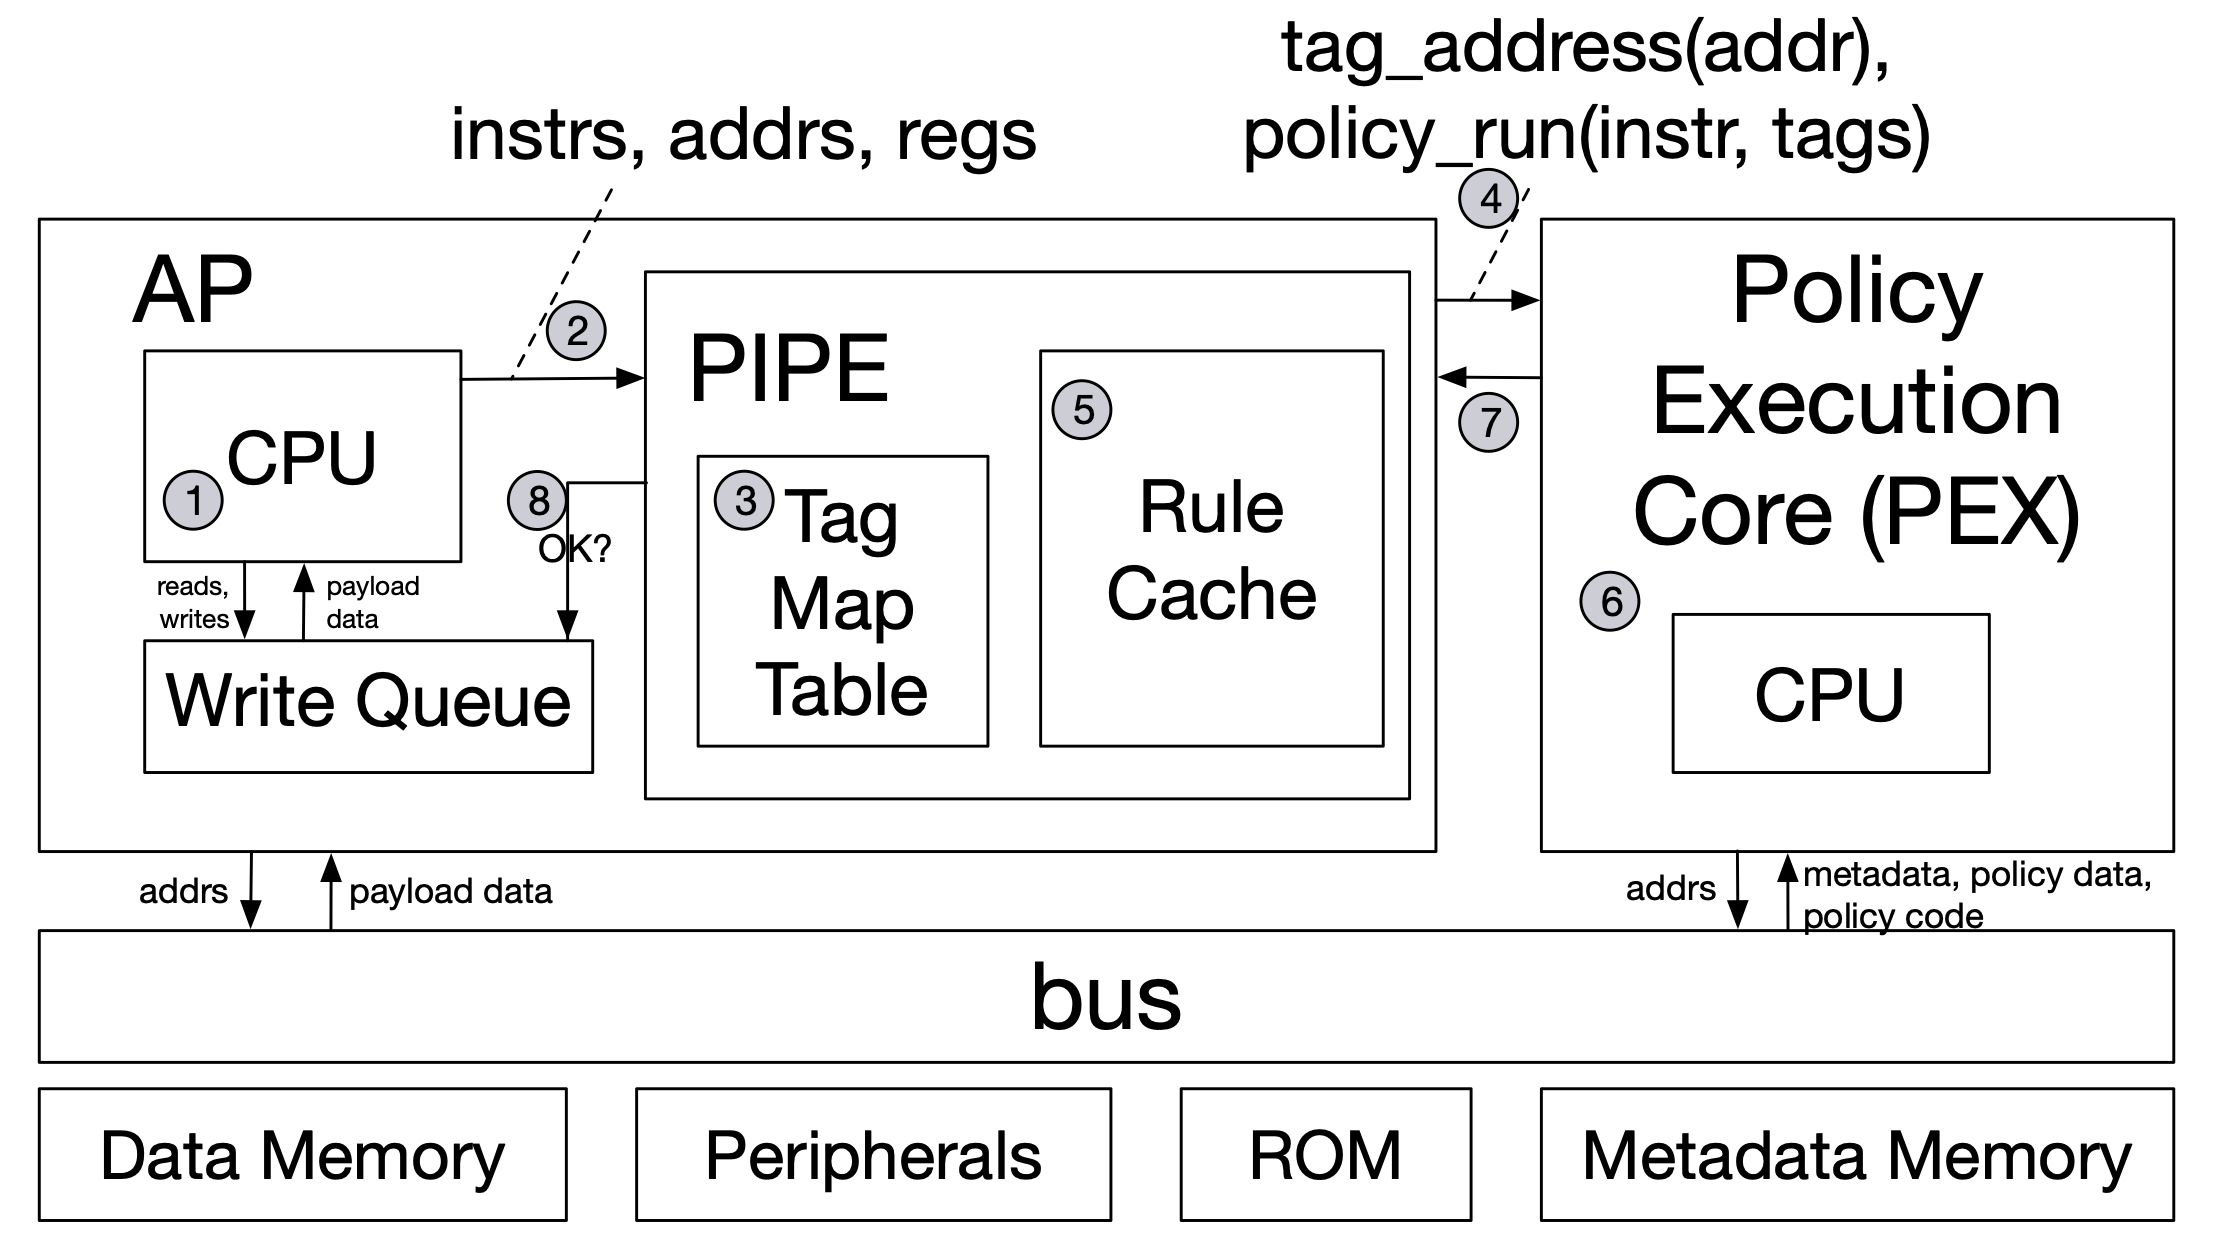
\includegraphics[width=0.8\textwidth]{Dover}
  \caption[Dover]{High level overview of Dover Architecture \cite{Dover}}
  \label{fig:Dover}
  \end{figure}x

%\subsection{Shakti-T}

%\subsection{HDFI}

%\subsection{lowRISC}

%\subsection{Taxi}

%\subsection{Pump}

\subsubsection{CHERI \cite{CHERI}}
CHERI (Capability Hardware Enhanced RISC Instructions) extends conventional processor
Instruction-Set Architectures (ISAs) with architectural capabilities to enable fine-grained
memory protection and highly scalable software compartmentalization. CHERI is a hybrid 
capability architecture that can combine capabilities with conventional MMU(i.e Memory Management
 Unit) based systems. The contribution of the following project include: 
\begin{itemize}
  \item ISA changes to introduce architecture capabilities.
  \item New microarchitecture proving that capabilities can be implemented efficiently 
        in hardware. Support for efficient tagged memory to protect capabilities and
        compress capabilities to reduce memory overhead.   
  \item Newly designed software construction model for that uses capability to provide
        fine grain memory protection and scalable software compartmentalization.  
  \item Language and Compiler extension to use capabilities for C and C++.
  \item OS extensions to use (and support application use of) fine-grained memory protection
        (spatial, referential, and (non-stack) temporal memory safety) and abstraction extensions
        to support scalable software compartmentalization. 
\end{itemize}

\begin{figure}[htbp!] 
  \centering    
  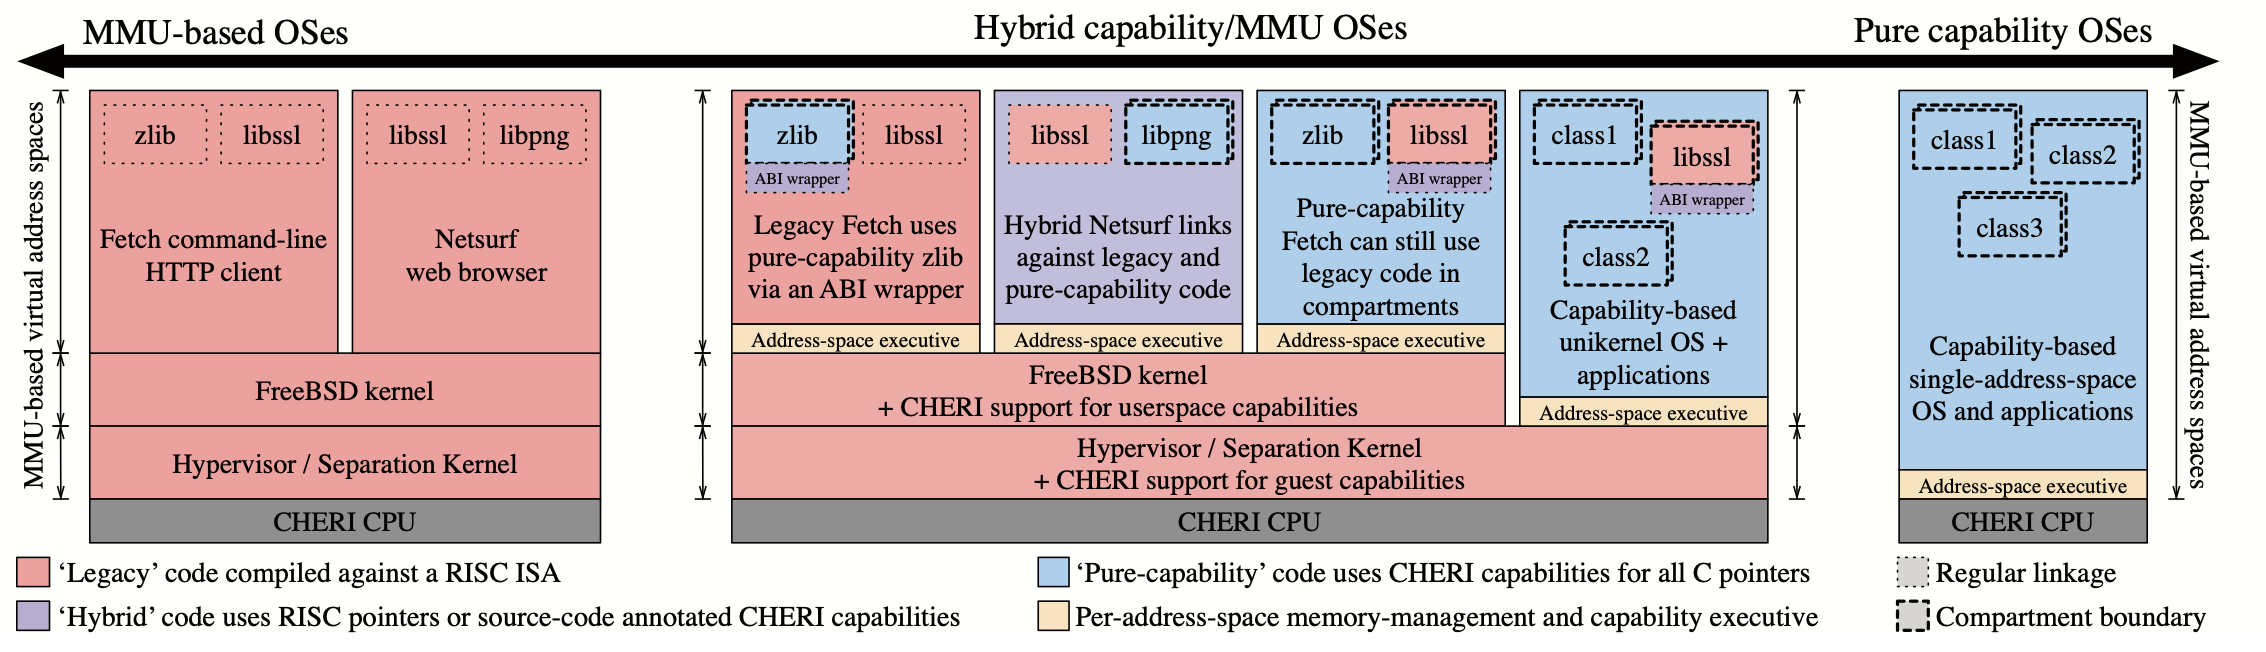
\includegraphics[width=0.9\textwidth]{Cheri}
  \caption[Cheri]{Spectrum of Hardware-software architectures, from conventional MMU-based virtualization and OS process models to single address-space capability system \cite{CHERI}}
  \label{fig:Cheri}
  \end{figure}
	
% \subsection{SPARC M7/M8 SSM}

\subsubsection{Low-Fat Pointers}
% https://dl.acm.org/doi/10.1145/2508859.2516713
Low-Fat Pointers\cite{LowFatPointer} adds hardware-managed tags to the pointer. 
This, in turn, allows the pointers to be used as capabilities to facilitate fine-grained 
access control and fast security domain crossing. The dedicated checking hardware runs in parallel 
with the processor's normal data-path so that the checks do not slow down processor operation 
(0\% runtime overhead).The following paper has a gate-level implementations of the logic for updating 
and validating these compact fat pointers and show that the hardware requirements are low 
and the critical paths for common operations are smaller than processor(i.e ALU operations).
The contribution of the following project include: 
\begin{itemize}
  \item Design and evaluation of a new, compact fat-pointer
  encoding and implementation (BIMA).
  \item Hardware that enforces the BIMA bounds checking and update, making the fat pointers 
  unforgeable and non-bypass able.
  \item Pipeline organization that allows the BIMA encoding to run just as fast as the baseline
   processor without spatial safety checking.
\end{itemize}


%\subsection{SAFE}

%\subsection{DataSafe}

%\subsection{Harmoni}

%\subsection{Shioya, et al.}

%\subsection{SIFT}

%\subsection{FlexCore}

%\subsection{Execution Leases}

%\subsection{GLIFT}

%\subsection{TIARA}

%\subsection{DIFT Coprocessor}

\subsubsection{HardBound}
% https://acg.cis.upenn.edu/papers/asplos08_hardbound.pdf
HardBound\cite{Hardbound} focuses on an architectural hardware bounded pointer primitive 
that supports hardware and software enforcements for memory safety in C programs. 
The C pointer representation is left intact but the bounds information is maintained 
separately and invisibly by the hardware. This means the bounds are initialized by 
software and is then propagated and transparently maintained by hardware (which automatically 
checks a pointer bound before it's dereferenced). The paper combined intra-procedural compiler 
instrumentation and hardware bounded pointers to enable a low overhead approach to enforce 
complete spatial memory safety in unmodified C programs. Based on the experiments conducted 
on the following paper the runtime overhead was between 5\% to 9\%. The following does not provide 
full type safety, handling dangling pointers and uninitialized memory reads.
The contribution of the following project include: 
\begin{itemize}
  \item A hardware bounded pointer primitive and accompanying complier transformation 
  that when combined enforce spatial safety for C programs. This is to minimize changes 
  to the compiler infrastructure and to retain compatibility with legacy C code. 
  \item Efficient implementation of hardware bounded pointers: This means using a compressed 
  metadata encoding, the entire base and metadata for bounds are stored in a reserver portion 
  of virtual memory. The hardware encodes the bounded pointer metadata by using just a few bits.
  These bits can be stored either in memory or unused bits in the pointer itself.
  \item Experimentally evaluating functional correctness and performance of the approach 
  in this paper.
\end{itemize}

% Evaluation (Hierarchy evaluation based on diagram provided in Survey)
% Choose either performance or Security 


% Concrete evaluation bring all together 
% - Combining multi-kernel with efficiency of Uni-kernels with Custom hardware to for type system checking.\\
% - Analyzing memory interleaving is also of interest. 



%\subsection{Loki}

%\subsection{FLexiTaint}

%\subsection{SECTAG}

%\subsection{Raksha}

%\subsection{SecureBit}

%\subsection{Minos}

% \subsection{DIFT}
% The following paper provides simple architectural mechanism called dynamic information 
% flow tracking. DIFT protects programs from malicious attacks by identifying phony information 
% from untrusted I/O and restricting the usage of the phony information.

%\subsection{RIFLE}

%\subsection{AEGIS}

%\subsection{Mondriaan}

%\subsection{Aries}

%\subsection{XOM}

%\subsection{M-Machine}

%\subsection{KCM}

%\subsection{SPUR}

%\subsection{Lisp Machine}

%\subsection{HEP}

%\subsection{Burroughs}






































